\chapter[Referencial Teórico]{Referencial Teórico}

Para inicializar o nosso Referencial teórico de forma concisa em que se alinhe com o que foi proposto com o capítulo 1, é imprescindível abordar o contexto e papel da Fertilização In Vitro, qualidade dos embriões e desafios associados, além de evidenciar como o Aprendizado de Maquina pode auxiliar a aprimorar as taxas de sucesso de gravidez e minimizar os fatores de risco relacionados a abortos, problemas cromossômicos, além de reduzir os impactos emocionais e físicos associados a esses desafios.

\section{Fertilização In Vitro}

A fertilidade tem sido um tema de grande relevância ao longo da história humana, visto como uma bênção divina em diversas culturas. Civilizações antigas, como a grega e a egípcia, realizavam rituais, usavam amuletos e talismãs, ou buscavam ajuda de divindades para garantir a continuidade de suas linhagens e prosperidade \cite{moura2020}. Esses métodos, embora enraizados em crenças religiosas e espirituais, refletem o desejo universal de superar desafios relacionados à reprodução.

Com os avanços científicos e médicos, a compreensão da fertilidade passou por uma profunda transformação. O primeiro marco documentado foi a inseminação artificial em animais, realizada pelos árabes em 1332 \cite{moura2020}. Essa técnica consiste na introdução do sêmen diretamente no sistema reprodutor da fêmea, otimizando as chances de fertilização \cite{corleta2010}. Em humanos, um dos eventos mais notáveis ocorreu em 1978, com o nascimento de Louise Brown, o primeiro "bebê de proveta" \cite{moura2020}. Este feito foi possível graças ao desenvolvimento da técnica de Fertilização In Vitro (FIV), criada pelo embriologista Robert Edwards e pelo ginecologista Patrick Steptoe. A técnica permitiu a fertilização de embriões fora do corpo humano e, por sua contribuição revolucionária, Edwards recebeu o Prêmio Nobel de Fisiologia ou Medicina em 2010 \cite{corleta2010}.

As Técnicas de Reprodução Assistida (TRA) compreendem um conjunto de métodos médicos especializados que buscam ajudar indivíduos com dificuldades reprodutivas a alcançarem a concepção \cite{souzamarise2024}. Dentre essas técnicas, a FIV se destaca como a mais avançada e amplamente utilizada \cite{moura2020}. O processo envolve várias etapas, como a estimulação ovariana controlada (uso de medicamentos para estimular a produção de óvulos), coleta de óvulos por punção transvaginal, fertilização em laboratório e posterior transferência dos embriões formados para o útero \cite{moura2020}.

Um avanço significativo no campo da TRA foi a introdução da Injeção Intracitoplasmática de Espermatozoides (ICSI), na década de 1990 \cite{pereira2016}. O ICSI é uma técnica complementar à FIV que consiste na injeção direta de um único espermatozoide no citoplasma do óvulo, utilizando uma micropipeta \cite{pereira2016}. Este método é particularmente útil em casos de infertilidade masculina severa, como baixa contagem de espermatozoides, baixa motilidade ou presença de anomalias estruturais nos espermatozoides \cite{pereira2016}. Embora a FIV possa ser realizada sem o uso de ICSI, este último é frequentemente empregado em casos que exigem maior precisão na fertilização \cite{pereira2016}.

Além de estabelecer as bases da medicina reprodutiva moderna, o nascimento de Louise Brown abriu caminho para avanços na medicina reprodutiva. Desde então, a combinação de avanços médicos e tecnológicos permitiu não apenas a realização da fertilização in vitro, mas também a análise genética detalhada dos embriões \cite{moura2020}. Esses exames identificam anomalias cromossômicas e genéticas, proporcionando uma maior chance de sucesso na implantação e no desenvolvimento de gestações saudáveis.

Os esforços históricos e as inovações científicas ilustram a busca contínua da humanidade por soluções eficazes contra a infertilidade. No próximo tópico, discutiremos detalhadamente a análise de embriões, um procedimento crucial para aumentar as chances de concepção saudável e seu papel na e seu papel na seleção de embriões para a FIV.

\section{Métodos de Avaliação Genética em Reprodução Assistida}

No contexto das Tecnologias de Reprodução Assistida, os métodos de avaliação genética desempenham um papel essencial na identificação de anomalias cromossômicas, como a aneuploidia, que é a alteração no número normal de cromossomos da espécie humana, representa a principal causa de falhas de implantação quando sua origem é embrionária. Dessa forma, a presença de aneuploidia nas células do embrião pode impactar diretamente a taxa de sucesso das técnicas de reprodução humana assistida. Além de dificultar a implantação, essa alteração cromossômica pode levar a abortos espontâneos ou até mesmo a malformações em bebês nascidos vivos \cite{milanezi2022}. Após décadas de avanços científicos, os testes genéticos tornaram-se cada vez mais precisos, com o desenvolvimento de técnicas sofisticadas e integradas à tecnologia, como a Testagem Genética Pré-implantacional.

Pelo final do século XX, o método do PGT começou a ser usado para realizar o rastreamento de doenças genéticas que possuíam uma alta taxa de incidência nas populações de amostra \cite{yang2024}. Com ele, foi propiciada a triagem de embriões antes da implantação, permitindo a seleção de embriões que possuíam menos riscos \cite{yang2024}. Tais métodos incluem a Testagem Genética Pré-implantacional para Doenças Monogênicas (PGT-M), como distrofia miotônica e fibrose cística; para rearranjos estruturais cromossômicos (PGT-SR); para aneuploidias (PGT-A), como Síndrome de Down e Síndrome de Turner; e mais recentemente, o PGT-P para doenças poligênicas \cite{yang2024}. No caso do nosso objeto de estudo, PGT-A, se destaca por sua capacidade de aumentar as chances de implantação embrionária bem-sucedida, reduzir a probabilidade de perdas gestacionais espontâneas e garantir maior probabilidade de nascimento de crianças com o número de cromossomos normais\cite{yang2024}. Além disso, o embrião considerado “normal” (euploide) apresenta 23 pares de cromossomos (46 cromossomos no total), sendo metade proveniente do espermatozoide e metade do óvulo. Já o embrião “anormal” (aneuploide) possui uma contagem incorreta de cromossomos em uma célula, sendo a maioria dos embriões com aneuploidias não compatíveis com a vida \cite{zegers2017}.

Os testes genéticos realizados durante a fase de blastocisto, formados cerca de 5{–}6 dias após a inseminação \cite{zegers2017}, são geralmente preferidos por especialistas em reprodução assistida porque essa abordagem envolve a coleta de células do trofectoderma, a camada externa do embrião que futuramente dará origem à placenta, e não diretamente do interior do embrião \cite{leaver2019}. Essa técnica, o PGT-A, é considerada menos invasiva em comparação com as biópsias realizadas na fase de clivagem, quando o embrião possui apenas algumas células e está em um estágio muito inicial de desenvolvimento \cite{leaver2019}. Na fase de clivagem, a retirada de células do interior do embrião (blastômeros), pode causar danos mais significativos ao embrião, afetando sua capacidade de se desenvolver adequadamente e reduzindo as chances de implantação bem-sucedida no útero \cite{leaver2019}. 

No entanto, é fundamental mencionar que a técnica de micromanipulação necessária para realizar esses procedimentos ainda não foi completamente padronizada. Isso significa que diferentes laboratórios podem adotar práticas distintas para a biópsia embrionária, o que pode resultar em variações na segurança e eficácia dos testes. Além disso, os impactos potenciais dessa intervenção, tanto nos desfechos reprodutivos (como taxas de gravidez e nascimento) quanto na saúde a longo prazo dos bebês nascidos a partir desses embriões, ainda não estão completamente compreendidos.

O PGT-A classifica os embriões em três categorias: euploide (normal, com 46 cromossomos), mosaico (mistura de células normais e anormais) e aneuploide (todas as células com número anormal de cromossomos). 
%A Figura~\ref{fig:ResultadosPGT} ilustra os resultados do PGT-A e suas respectivas probabilidades de sucesso gestacional.

\begin{center}
    \begin{figure}[h]
        \captionsetup{font=footnotesize, position=above}
        \caption{Resultados do PGT-A e suas respectivas probabilidades de sucesso gestacional}
        \label{fig:ResultadosPGT}
        \centering
        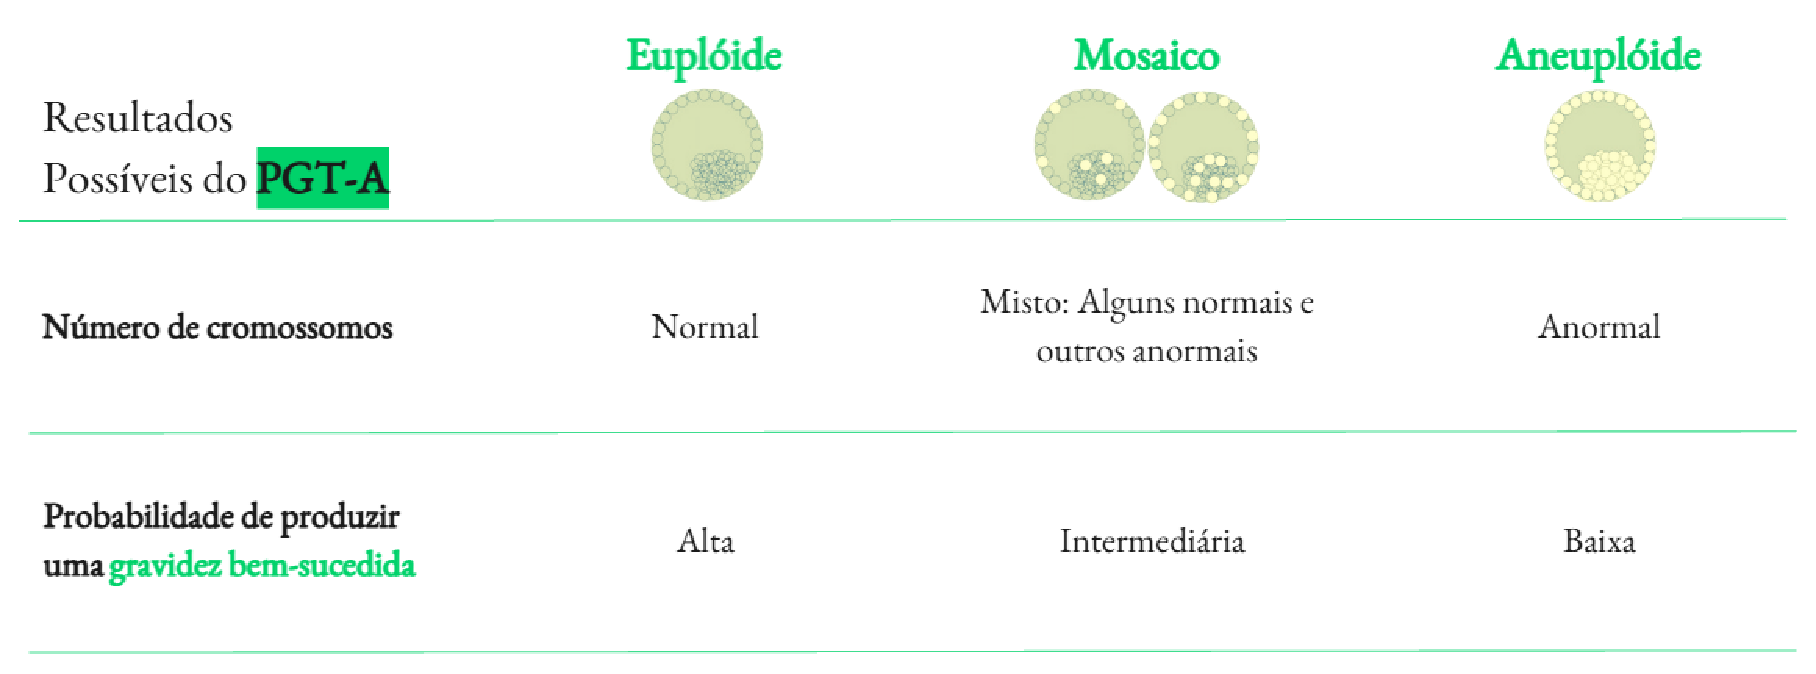
\includegraphics[scale=0.5]{figuras/ResultadosPGT.pdf}
        \vspace{0.3cm} 
        % \caption{Classificação dos embriões após o teste genético pré-implantacional para aneuploidias (PGT-A). O PGT-A avalia o número de cromossomos em células do embrião, permitindo classificá-los em três categorias: euploides (número normal de cromossomos), mosaicos (mistura de células com número normal e anormal de cromossomos) e aneuploides (número anormal de cromossomos em todas as células). A figura ilustra esquematicamente as diferentes classificações e as respectivas probabilidades de sucesso gestacional.}
        % \scriptsize{Classificação dos embriões após o teste genético pré-implantacional para aneuploidias (PGT-A). O PGT-A avalia o número de cromossomos em células do embrião, permitindo classificá-los em três categorias: euploides (número normal de cromossomos), mosaicos (mistura de células com número normal e anormal de cromossomos) e aneuploides (número anormal de cromossomos em todas as células). A figura ilustra esquematicamente as diferentes classificações e as respectivas probabilidades de sucesso gestacional.}
    \end{figure}
\end{center}
\FloatBarrier

Apesar de suas vantagens, o PGT-A apresenta limitações significativas, como a variabilidade nos resultados das biópsias do trofectoderma e o risco de diagnósticos falso-positivos \cite{gleicher2021}. A The Preimplantation Genetic Diagnosis International Society (PGDIS) e a European Society of Human Reproduction and Embryology (ESHRE) apontam questões críticas, incluindo:

\begin{itemize}
    \item As divergências no conteúdo de DNA aneuploide entre diferentes regiões da trofoectoderma e a massa celular interna demonstram que a biópsia de cinco células pode apresentar resultados variados;
    \item O número exato de células na biópsia nunca é conhecido, o que impossibilita determinar com precisão a porcentagem de DNA aneuploide;
    \item A biópsia da trofoectoderma danifica células individuais, causando vazamento de DNA e contaminação das células vizinhas, dificultando a medição precisa da aneuploidia;
    \item O limiar de 20\% entre euploidia e mosaicismo é baseado apenas na sensibilidade atual do sequenciamento de nova geração (NGS), que não detecta níveis inferiores a 20\% de DNA aneuploide. Consequentemente, qualquer mosaicismo abaixo de 20\% é considerado euploide normal;
    \item Dentro da faixa de mosaicismo (20\% a 80\%), os desfechos de implantação e nascimento são semelhantes, indicando que o uso de limiares rígidos para predizer resultados de FIV é incorreto.
\end{itemize}

Estudos indicam que embriões descartados como aneuploides pelo PGT-A resultaram em nascimentos normais \cite{gleicher2021}, evidenciando a necessidade de revisar as diretrizes para evitar o desperdício de embriões viáveis. A figura abaixo ilustra a seleção de um pedaço do embrião e como isso pode influenciar a definição da ploidia do mesmo. A biópsia mencionada nas etapas do PGT-A, envolvendo a remoção de uma célula do embrião para análise genética \citeonline{phillips2024}, levantam a preocupação de que a remoção dessas células em crescimento possa comprometer o desenvolvimento do embrião, afetando os resultados neonatais, visto que as técnicas de micromanipulação utilizadas na biópsia não são totalmente isentas de riscos, como observado por \citeonline{leaver2019}.

\begin{figure}[h]
    \captionsetup{font=footnotesize, position=above}
    \caption{Discrepância potencial entre uma biópsia de células utilizando PGT-A e a composição celular em regiões adjacentes do trofectoderma}
    \label{fig:biopsiaPGT-A}
    \centering
    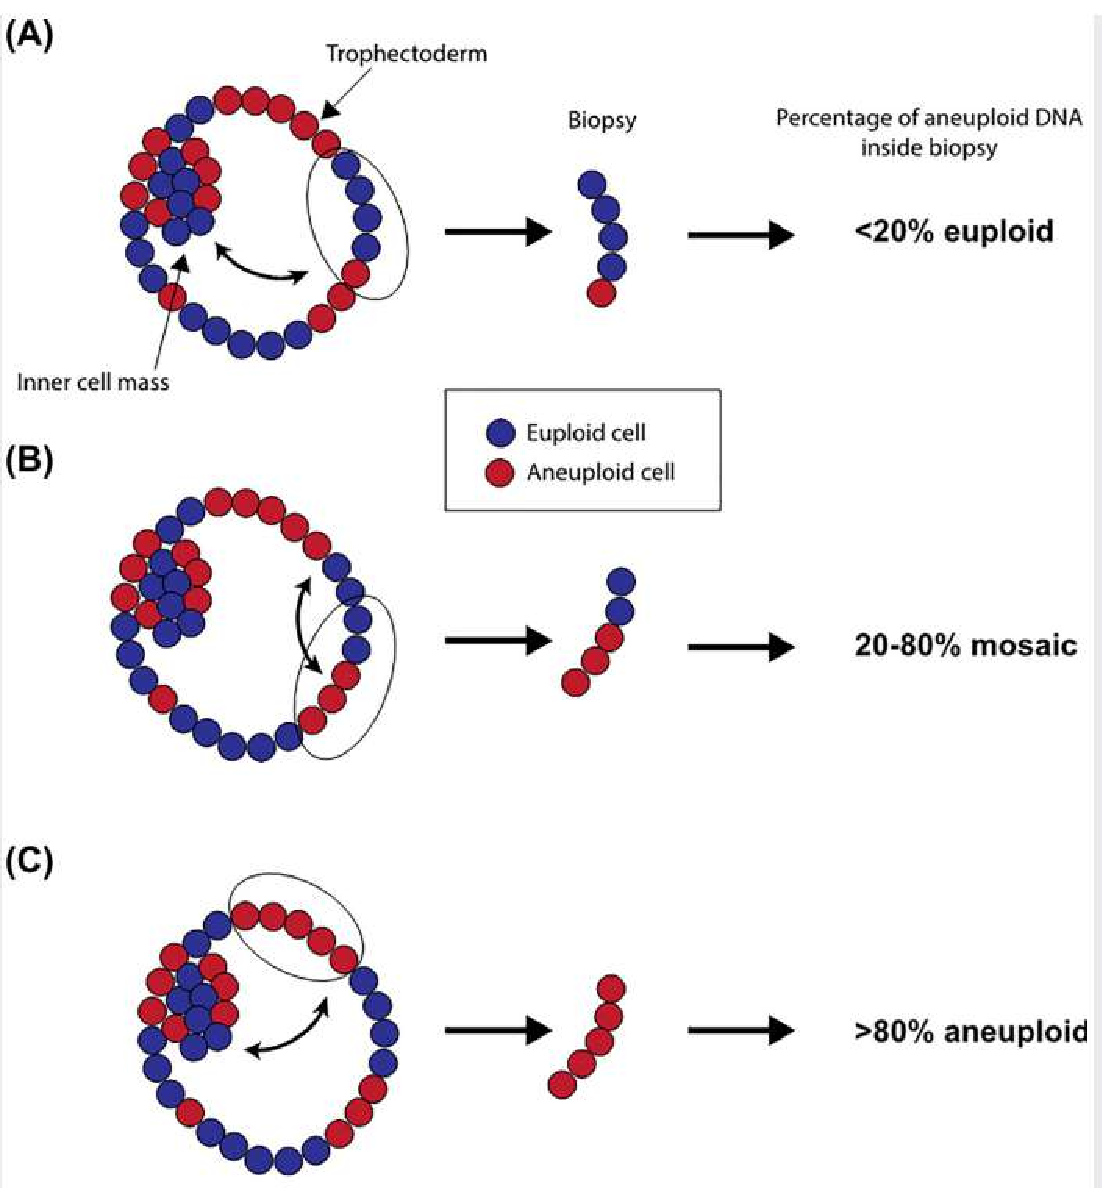
\includegraphics[scale=0.6]{figuras/biopsiaPGT-A.pdf}
    \vspace{0.3cm} 
    \begin{minipage}{\linewidth}
        \centering
        % \caption{Representação esquemática da biópsia do trofectoderma e a influência da amostragem na determinação da ploidia embrionária. (A) Embrião euploide com células da massa celular interna (MCI) e do trofectoderma (TE) com pouca ou nenhuma aneuploidia. A biópsia resulta em uma amostra com menos de 20\% de células aneuploides, classificando o embrião como euploide. (B) Embrião mosaico com proporção similar de células euploides e aneuploides. A biópsia pode resultar em uma amostra com 20-80\% de células aneuploides, classificando o embrião como mosaico. (C) Embrião predominantemente aneuploide. A biópsia resulta em uma amostra com mais de 80\% de células aneuploides, classificando o embrião como aneuploide. Observação: A ploidia embrionária determinada pela biópsia do trofectoderma pode variar de acordo com a região amostrada, devido à mosaicidade embrionária. A figura ilustra a incerteza associada à classificação da ploidia embrionária com base em uma pequena amostra de células.}
        % \scriptsize{Representação esquemática da biópsia do trofectoderma e a influência da amostragem na determinação da ploidia embrionária. (A) Embrião euploide com células da massa celular interna (MCI) e do trofectoderma (TE) com pouca ou nenhuma aneuploidia. A biópsia resulta em uma amostra com menos de 20\% de células aneuploides, classificando o embrião como euploide. (B) Embrião mosaico com proporção similar de células euploides e aneuploides. A biópsia pode resultar em uma amostra com 20-80\% de células aneuploides, classificando o embrião como mosaico. (C) Embrião predominantemente aneuploide. A biópsia resulta em uma amostra com mais de 80\% de células aneuploides, classificando o embrião como aneuploide. Observação: A ploidia embrionária determinada pela biópsia do trofectoderma pode variar de acordo com a região amostrada, devido à mosaicidade embrionária. A figura ilustra a incerteza associada à classificação da ploidia embrionária com base em uma pequena amostra de células.}
    \end{minipage}
\end{figure}
\FloatBarrier

Embora o PGT-A permita detectar aneuploidias e aumente as chances de uma gravidez bem-sucedida, ele pode impactar negativamente o potencial de implantação do embrião \cite{gleicher2021}. Por esses motivos, métodos não invasivos estão sendo estudados como alternativas eficientes e seguras, tornando-se cada vez mais relevantes. Um exemplo de técnica não invasiva é a análise morfocinética a partir de imagens obtidas de incubadoras de última geração equipadas com a tecnologia Time-Lapse System.

\section{Time-Lapse System}

O TLS é um sistema que captura imagens contínuas dos embriões em desenvolvimento, em intervalos regulares, sem alterar o ambiente de cultivo \cite{moustakli2024}. Essa análise morfocinética, gerada pelas imagens adquiridas pelo TLS, permite o monitoramento quase contínuo do desenvolvimento do embrião, possibilitando a observação de eventos dinâmicos e frequentemente transitórios que não seriam visíveis em observações estáticas \cite{boucret2021}. O uso do TLS não interrompe as condições de cultura, mantendo a viabilidade do embrião durante o processo de monitoramento \cite{moustakli2024}.

As variáveis morfocinéticas incluem aspectos como a forma e a estrutura do embrião (morfológicas) e o movimento e o desenvolvimento do embrião ao longo do tempo (cinéticas), os quais são essenciais para uma análise detalhada de seu progresso \cite{gleicher2021}. Com esse monitoramento contínuo, é possível observar a regularidade das divisões celulares e identificar momentos críticos do crescimento, o que pode auxiliar na diferenciação de embriões euplóides e aneuplóides com base no seu padrão de desenvolvimento \cite{boucret2021}. De acordo com \citeonline{moustakli2024}, o TLS oferece insights valiosos sobre a saúde e o potencial de desenvolvimento dos embriões, utilizando uma abordagem não invasiva, em contraste com a biópsia de embriões. Alguns estudos indicam que, ao ser combinado com pontuações morfocinéticas, o TLS pode aumentar as taxas de implantação e gravidez clínica em comparação aos métodos tradicionais \cite{boucret2021}.

As variáveis da planilha de dados, dados esses extraídos pelo TLS, que estamos utilizando para esse trabalho incluem informações sobre a qualidade morfológica e cinética dos embriões, como a taxa de divisão celular e a regularidade do desenvolvimento, . Essas variáveis são essenciais para a análise morfocinética e a classificação dos embriões em diferentes estágios de desenvolvimento \cite{boucret2021}. A seguir, discutiremos as variáveis cientificamente comprovadas que influenciam a ploidia.

\subsection{Idade}

As informações trazidas pelo Fertility and Ageing (\citeonline{eshre2005}) corroboram a relevância de incluir variáveis relacionadas à \textbf{idade materna}, pois estudos apontam que o aumento da aneuploidia em embriões está diretamente associado ao envelhecimento materno. O estudo de \citeonline{yuan2023} aponta que a taxa de euploidia dos embriões está correlacionada com a idade feminina. À medida que a idade avança, há um declínio no número total e na qualidade dos ovócitos, um fator crítico para a fecundidade reduzida observada após os 35 anos \cite{yuan2023}. Além disso, a resposta à estimulação ovariana e os níveis de FSH (hormônio folículo-estimulante) emergem como possíveis variáveis preditivas relevantes. Estudos indicam que a idade materna exerce maior influência sobre a qualidade embrionária do que os níveis de FSH isoladamente, reforçando que o impacto na fertilidade está mais relacionado à qualidade do oócito do que à sua quantidade \cite{eshre2005}.

\subsection{t2, t3, t4, t5, t8, s2, cc2 (t3-t2), tSC, tSB, tB, cc3 (t5-t3), s3 (t8-t5), t5-t2,  tSC-t8 e tB-tSB}

Os \textbf{sistemas de Time-Lapse} ajudam a identificar \textbf{marcadores morfocinéticos}, que mostram como as células se dividem durante o desenvolvimento do embrião. Esses marcadores, junto com características físicas tradicionais, são fundamentais para selecionar o embrião mais adequado para a transferência \cite{souzarebeca2022}. O desenvolvimento embrionário é um processo dinâmico, com mudanças perceptíveis em um curto período \cite{cruz2012}. Estudos detalhados sobre o ritmo das divisões celulares, assim como características como tamanho e organização das células, demonstram que o tempo necessário para atingir certos estágios de desenvolvimento está diretamente relacionado ao potencial de implantação do embrião \cite{souzarebeca2022}.

Embriões que se dividem muito rapidamente apresentam menor chance de implantação quando comparados aos que seguem um ciclo celular dentro do intervalo considerado normal \cite{cruz2012}. Isso ocorre porque alterações no tempo de compactação inicial, na formação da blástula e na progressão até o estágio de blastocisto completo estão associadas a uma maior probabilidade de aneuploidias \cite{cruz2012}. O projeto \textit{Timing of cell division in human cleavage-stage embryos is linked with blastocyst formation and quality} de \citeonline{cruz2012} utilizou o sistema Time-Lapse para identificar marcadores morfocinéticos e monitorar com precisão os tempos das divisões celulares durante o desenvolvimento embrionário. Os tempos considerados ótimos para previsões de desenvolvimento embrionário foram: \textbf{t2 (24,3{–}27,9 horas), t3 (35,4{–}40,3 horas), t5 (48,8{–}56,6 horas), s2 (<0,76 horas) e cc2 (<11,9 horas)}. A explicação detalhada dessas variáveis está disponível no \textbf{Apêndice \ref{apendice:variaveis}}.

Especificamente, no nível morfológico, \textbf{t5} destacou-se como o indicador mais relevante do potencial de implantação \cite{cruz2012}. Observa-se que a capacidade de diferenciar embriões viáveis daqueles não viáveis melhora significativamente quando os critérios se baseiam em eventos de divisão celular mais tardios \cite{cruz2012}. Embriões com t5 entre 48,8 e 56,6 horas demonstram não apenas um maior potencial de implantação, mas também uma maior propensão a se desenvolverem em blastocistos de morfologia superior \cite{cruz2012}.

Ao criar um modelo de IA para a previsão de euploidia, é importante que considere as variáveis \textbf{t4, t8, tSC, tSB, tB, cc3 (t5 - t3) e s3 (t8 - t5)}. Essas métricas são fundamentais para o desenvolvimento embrionário, conforme evidenciado no estudo que comprovou a efetividade da IA em detectar embriões viáveis com uma precisão de 70\% \cite{rienzi2020}. A incorporação dessas variáveis em um modelo de IA é crucial, pois possibilita a captura das sutilezas do desenvolvimento embrionário, que, de acordo com a pesquisa, são melhoradas através da análise automatizada fundamentada em Inteligência Artificial. Isso se torna especialmente relevante pois os sistemas de time-lapse disponibilizam informações detalhadas e contínuas, que podem ser combinadas para detectar padrões relacionados à euploidia \cite{rienzi2020}.

A avaliação de fatores morfocinéticos, como o tempo necessário para clivagem e a extensão das fases subsequentes, tem sido alvo de pesquisa para antecipar a probabilidade de implantação embrionária. Por exemplo, um estudo publicado pelo Instituto Sapientiae por \citeonline{desai2019} destacou a importância desses parâmetros na predição do potencial de implantação embrionária. Apesar dessa pesquisa não tratar especificamente os intervalos \textbf{t5-t2, tSC-t8 e tB-tSB}, ela sugere que a avaliação de intervalos de tempo entre eventos específicos no desenvolvimento embrionário pode oferecer percepções valiosas sobre a qualidade e a capacidade de desenvolvimento dos embriões \cite{desai2019}.

\subsection{Estágio e Morfo}

Modelos de IA têm sido empregados na avaliação de embriões produzidos até o quinto dia ou mais, com o objetivo de aprimorar a escolha com base em informações objetivas e de alta exatidão \cite{lassen2022}. Esses modelos priorizam a análise dos estágios "\textbf{Dia 5+}", ou seja, aqueles que atingem o estágio de blastocisto no quinto dia ou mais tarde, devido à maior disponibilidade de dados morfológicos e dinâmicos do desenvolvimento embrionário \cite{lassen2022}. 

De acordo com os critérios definidos por \citeonline{gardner1999}, com base na \textbf{morfologia do embrião} se tem a categorização dos blastocistos, um fator determinante para o potencial de implantação e a qualidade embrionária \cite{capalbo2014}. Os blastocistos são agrupados em quatro categorias principais, considerando tanto a massa celular interna (ICM, Inner Cell Mass) quanto o TE (trophectoderma):
\begin{itemize}
  \item \textbf{Grupo 1 (Excelente)}: Blastocistos com classificação  \textbf{$\geq$ 3AA}. Blastocistos altamente desenvolvidos com massa celular interna densa e trophectoderma bem organizado \cite{capalbo2014}.
  \item \textbf{Grupo 2 (Bom)}: Blastocistos com classificação \textbf{3, 4, 5 ou 6} e com notas \textbf{AB ou BA}. Apresentam características boas, mas menos consistentes em relação ao grupo excelente \cite{capalbo2014}.
  \item \textbf{Grupo 3 (Médio)}: Blastocistos com classificação \textbf{3, 4, 5 ou 6} e notas \textbf{BB, AC ou CA}. Qualidade moderada com irregularidades tanto na ICM quanto no TE \cite{capalbo2014}.
  \item \textbf{Grupo 4 (Ruim)}: Blastocistos com classificação \textbf{$\leq$ 3BB}.Blastocistos de menor qualidade, com poucas células organizadas na ICM e TE menos coeso \cite{capalbo2014}.
\end{itemize}
O estudo de \citeonline{capalbo2014} enfatizou a relação entre a morfologia padrão dos blastocistos, a euploidia e as taxas de implantação. Blastocistos de excelente morfologia, particularmente os biopsiados no dia 5, mostraram uma maior probabilidade de serem euploides e apresentaram taxas de implantação superiores.

\subsection{KIDScore\texttrademark}  

O KIDScore\texttrademark{}, um algoritmo baseado em IA aplicado à análise de imagens em sistemas Time-Lapse, tem se mostrado uma ferramenta importante na avaliação de embriões durante os tratamentos de reprodução assistida \cite{kato2021}. O algoritmo combina variáveis morfocinéticas e parâmetros de desenvolvimento embrionário para fornecer uma pontuação que auxilia na seleção de embriões com maior potencial de implantação e viabilidade genética \cite{gazzo2020}. A pontuação vai de \textbf{0 a 10}. Pontuações baixas, entre 0 e 3, indicam embriões de qualidade inferior, com baixo potencial de implantação. Pontuações médias, de 4 a 6, correspondem a embriões de qualidade moderada, com um potencial razoável de implantação. Já pontuações altas, de 7 a 10, representam embriões de alta qualidade, com grande potencial de implantação \cite{gazzo2020}. \citeonline{kato2021} cita que o modelo apresentou uma alta precisão na previsão de resultados de gravidez, sendo especialmente útil tanto em pacientes com idade materna avançada quanto em pacientes mais jovens. Por fim, \citeonline{gazzo2020} informaram que o uso do algoritmo no processo de seleção embrionária levou a um aumento expressivo nas taxas de implantação após a transferência de embriões congelados (FET). Então o modelo quando combinada com informações sobre os tempos de divisão celular, sendo \textbf{t2, t3, t5, s2 e cc2} descritos por \citeonline{cruz2012}, possibilita um exame mais completo do crescimento embrionário, melhorando a acurácia na seleção de embriões com maior probabilidade de êxito em tratamentos de FIV.

\subsection{Ploidia}
Para a elaboração do nosso modelo de previsão de euploidia, optamos por empregar a coluna de \textbf{Ploidia}, que proporciona uma categorização minuciosa dos embriões em diversas categorias de euploidia. As categorizações contidas nesta coluna são: Aneuploide complexo, Aneuploide/Triploide XXX, Caótico, Haploide, Mosaico de alto grau, Mosaico de baixo grau e Normal/Euploide. De acordo com o \citeonline{bastida2019}, considera-se os embriões com Caótico, Haplóide e Mosaico de alto grau como Aneuploides, enquanto os com mosaico de baixo grau como Euploides. Diante disso, optamos por reorganizar os valores na tabela de dados, agrupando as seguintes categorias sob o termo \textbf{Aneuploide}: Aneuploide complexo, Aneuploide/Triploide XXX, Caótico, Haploide e Mosaico de alta complexidade. Em contrapartida, os embriões categorizados como Mosaico de baixo grau e Normal/Euploide serão reunidos na categoria \textbf{Euploide}.

\section{Aprendizado de Máquina}

As dificuldades em definir IA não são, portanto, o resultado de alguma deficiência ou descuido, mas surgem do fato de que fomos incapazes de determinar precisamente qual inteligência desejaríamos replicar artificialmente \cite{sheikh2023}. Dessa forma, definimos a Inteligência Artificial como sistemas que exibem comportamento inteligente ao analisar seu ambiente e tomar ações {–} com algum grau de autonomia {–} para atingir objetivos específicos \cite{sheikh2023}. 

Na medicina reprodutiva, a IA tem se mostrado promissora na melhoria de processos como a fertilização in vitro (FIV). Essa busca por imitar a inteligência humana e entender seus processos cognitivos levou ao desenvolvimento de diversas abordagens, entre elas o Aprendizado de Máquina (Machine Learning, ML), que envolve a capacidade de computadores de interpretar grandes volumes de dados, construir modelos baseados nesses dados e, assim, gerar hipóteses ou previsões sobre o mundo ao seu redor \cite{russell2016}. Na medicina, algoritmos podem ser treinados para reconhecer padrões genéticos em embriões, classificar o melhor embrião para implantação e prever características genéticas de novos embriões. 

Os métodos de ML são geralmente classificados em três tipos principais: aprendizado supervisionado, aprendizado não supervisionado e aprendizado por reforço. Neste estudo, opta-se pelo aprendizado supervisionado como abordagem principal, dada sua eficácia na análise de dados rotulados, permitindo decisões mais precisas e embasadas para otimizar os tratamentos de FIV.

O aprendizado supervisionado consiste no treinamento de algoritmos com base em conjuntos de dados rotulados, nos quais as variáveis de entrada (inputs) e os resultados esperados (outputs) já são conhecidos. O algoritmo aprende a correlacioná-los de forma eficiente \cite{russell2016}, ajustando seus parâmetros com base nas diferenças entre previsões e resultados reais \cite{trask2019}. Uma técnica amplamente usada dentro do aprendizado supervisionado é a classificação, cujo objetivo é atribuir rótulos ou classes pré-definidas aos dados. Por exemplo, no contexto da medicina reprodutiva, um modelo pode ser treinado para diferenciar embriões euploides e aneuploides, aprendendo a reconhecer padrões associados a cada grupo \cite{izbicki2020}.

\begin{figure}[h]
    \captionsetup{font=footnotesize, position=above}
    \caption{Aprendizado Supervisionado: Identificando Euploidia e Aneuploidia}
    \label{fig:biopsiaPGT-A}
    \centering
    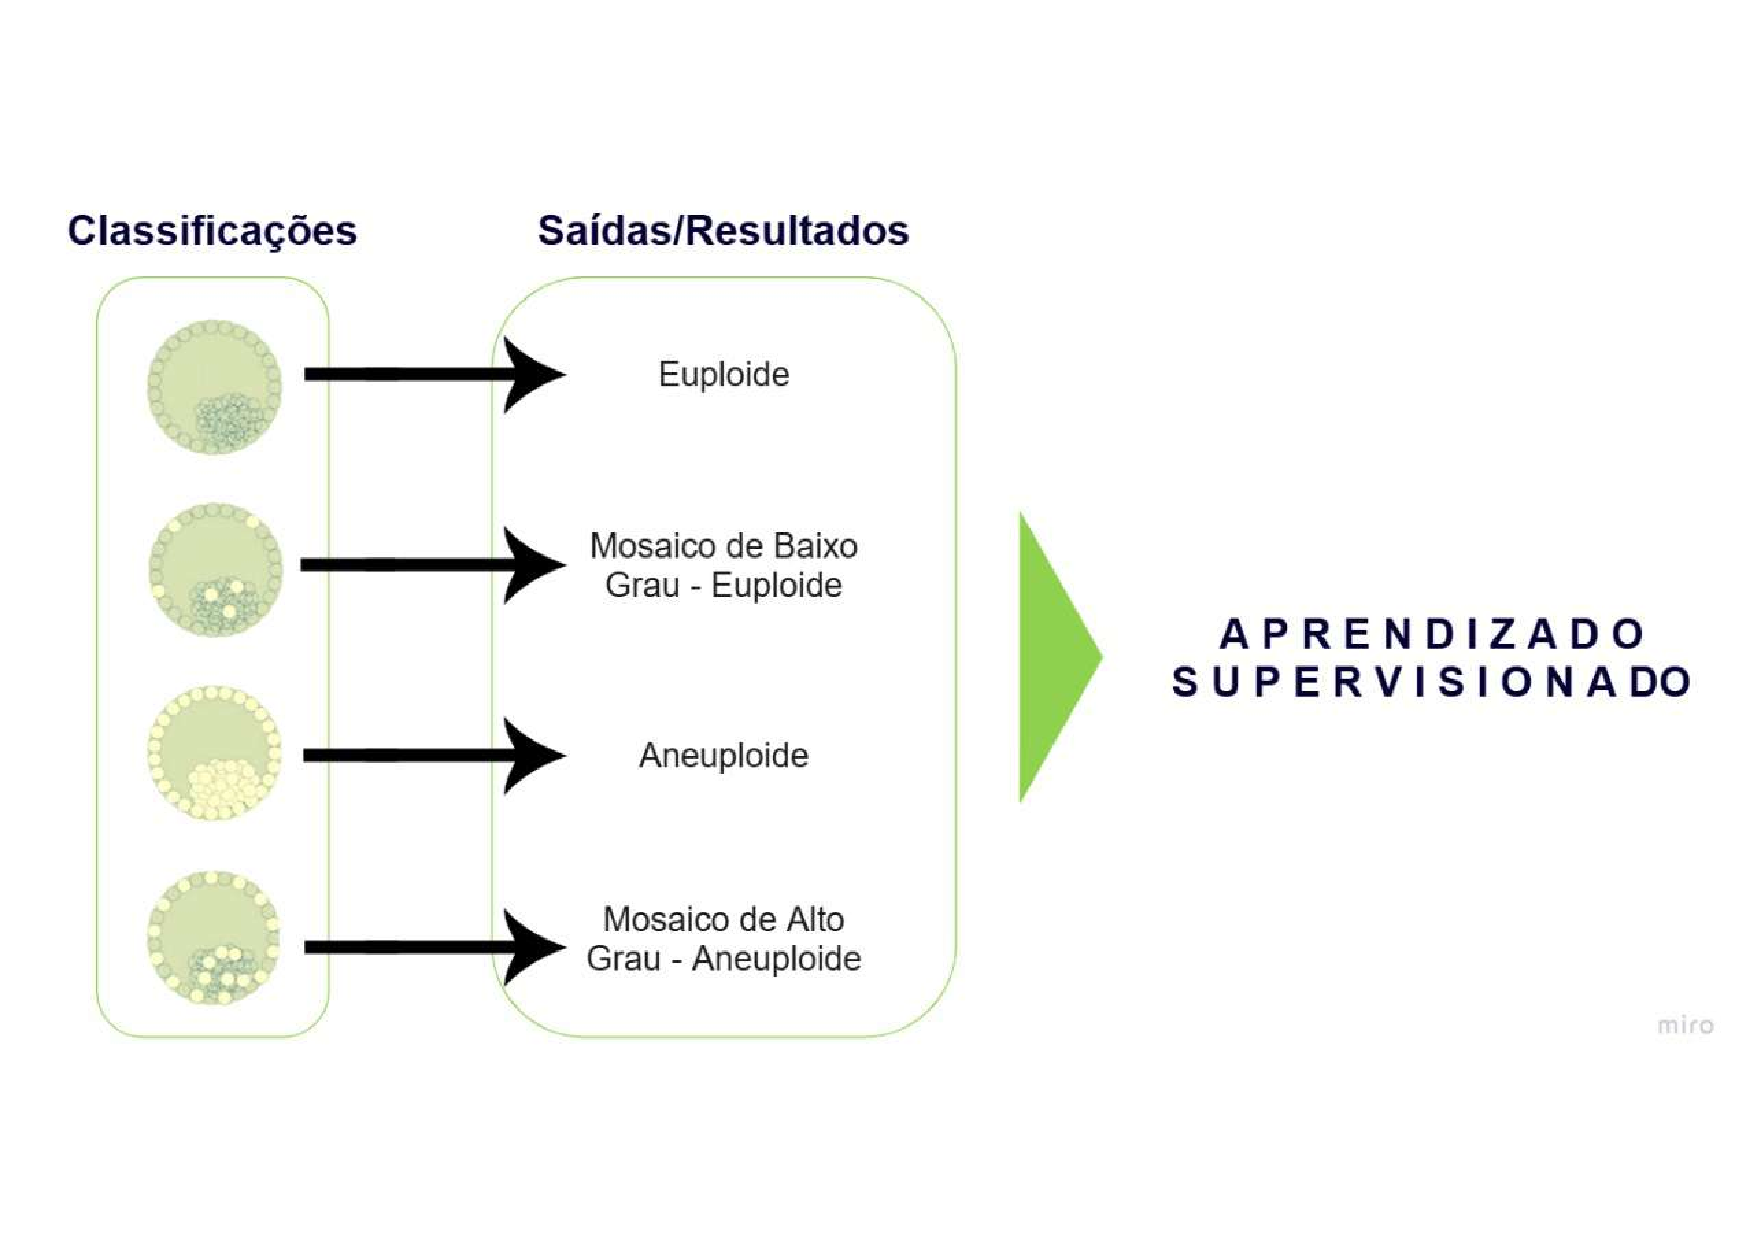
\includegraphics[scale=0.35]{figuras/aprendizadoSuper.pdf}
    \vspace{0.3cm} 
    % \caption{Os dados já possuem seus próprios rótulos. Já é definido o que significa ser euploide e aneuplóide. Os dados rotulados (ou seja, com rótulos já atribuídos) são usados para treinar o modelo. Nesse contexto, ao se referir a "euploide" e "aneuplóide", esses rótulos podem representar classes que o modelo deve aprender a identificar com base nas características dos dados, ajudando a prever ou classificar novos casos com precisão.}
\end{figure}
\FloatBarrier

De maneira geral, um algoritmo de aprendizado supervisionado separa o banco de dados em três subconjuntos: treinamento, validação e teste \cite{izbicki2020}. Na fase de treinamento, o algoritmo identifica padrões nos dados de entrada e os associa às classes desejadas \cite{izbicki2020}. Na validação, um subconjunto de dados não utilizado no treinamento avalia o desempenho do modelo \cite{izbicki2020}, permitindo ajustes nos hiperparâmetros. Após resultados satisfatórios, o conjunto de testes mensura métricas como acurácia, recall e precisão, garantindo o desempenho esperado \cite{izbicki2020}.

A seleção aleatória das amostras para treinamento, validação e teste é uma boa prática \cite{izbicki2020}, evitando problemas decorrentes de ordenações previamente estabelecidas nos bancos de dados. Isso assegura uma visão representativa e imparcial dos dados, fundamental para a construção de modelos robustos e confiáveis \cite{izbicki2020}.

Para a exploração inicial dos dados, utilizaremos o modelo k-Nearest Neighbors (kNN) como ponto de partida, conforme apresentado no livro Aprendizado de Máquina: Uma Abordagem Estatística \citeonline{izbicki2020}. Caso o desempenho e a confiabilidade do kNN não sejam satisfatórios, passaremos a avaliar outros modelos de classificação, como Regressão Linear e Naive Bayes, seguindo esse processo iterativo até encontrarmos um modelo que atenda aos critérios desejados. Se alguns desses modelos demonstrarem resultados satisfatórios, não será necessário explorar os demais.

\subsection{O Algoritmo K-Nearest Neighbor}

O algoritmo K-Nearest Neighbor (KNN) é, em essência, um dos algoritmos mais simples e populares em aprendizado supervisionado, sendo utilizado principalmente em tarefas de classificação e regressão \cite{zhang2016}. Sua principal característica é classificar uma nova observação com base nas classes de seus k vizinhos mais próximos previamente rotulados \cite{zhang2016}. O KNN pode ser considerado um modelo não paramétrico, pois não faz suposições a respeito da distribuição dos dados, o que o torna bastante versátil para uma diversidade de problemas \cite{zhang2016}. É também um algoritmo de aprendizado "preguiçoso" já que não ocorre um processo explícito de aprendizado \cite{zhang2016}.  Então, o algoritmo armazena os dados de treinamento e, na hora de fazer uma predição usa a distância da nova observação para cada exemplo discretamente do conjunto de treinamento para descobrir qual classe ou valor alvo deve usar \cite{zhang2016}.

O desempenho do KNN dé dependente da escolha de k, que são o número de vizinhos que são considerados na classificação \cite{zhang2016}. Valores muito pequenos de k podem a levar a overfitting, já que o modelo se torna sensível ao ruídos contidos nos dados. Valores muito grandes, por sua vez, podem resultar em underfitting pela perda de padrões locais importantes \cite{elkan2011}. Nesse trabalho, utilizaremos num primeiro momento k = 3 e k = 5 para avaliar o desempenho do modelo. Estes valores são adequados uma vez que eles capturam padrão locais sem exagerada sensibilidade ao ruído. Caso necessário, faremos o ajuste no parâmetro k com base nos resultados do conjunto de validação, pois o conjunto de validação é empregado especificamente para otimizar hiperparâmetros.

A métrica de distância adotada foi a distância Euclidiana, uma das mais simples e mais utilizadas. Essa é uma escolha adequada para pequenos conjuntos de dados e de baixa dimensionalidade, como o utilizado neste estudo. Para tais condições a distância euclidiana capta similaridades com eficiência, além de facilitar a interpretação dos resultados \cite{elkan2011}.

O funcionamento do KNN pode ser resumido em três etapas principais de acordo com o \citeonline{elkan2011}:
\begin{itemize}
    \item Armazenar os exemplos de treinamento com suas respectivas etiquetas.
    \item Calcular a distância entre uma nova observação e todos os exemplos armazenados, utilizando uma métrica de similaridade, como a distância Euclidiana.
    \item Selecionar os k vizinhos mais próximos e determinar a classe mais frequente entre eles, atribuindo-a à nova observação.
\end{itemize}

Essa abordagem de classificação por maioria contribui para mitigar o impacto de ruídos ou valores extremos \cite{elkan2011}. Uma prática comum para definir o valor de k é utilizar a raiz quadrada do número total de observações no conjunto de treinamento, embora ajustes específicos sejam feitos dependendo do problema e do conjunto de dados \cite{elkan2011}.

\subsection{Regressão Linear}

A regressão linear é uma técnica estatística utilizada em aprendizado de máquina para expressar relações entre variáveis e para realizar previsões baseadas em dados passados \cite{rodrigues}. É uma abordagem essencial em aprendizado supervisionado, oque visa detectar padrões e criar modelos generalizáveis para dados até então inexistentes \cite{soto}. Segundo \citeonline{santos2007},  é usada para quantificar a associação entre as variáveis, usando frequentemente o coeficiente de correlação de Pearson para avaliar a força e a direção dessa relação. A regressão linear pode ser dividida em dois tipos principais: regressão linear simples e regressão linear múltipla \cite{soto}.

Em um contexto de IA, a regressão linear simples estabelece uma relação matemática entre uma variável dependente \( Y \) e uma única variável independente \( X \), descrita pela equação:
\[
Y = \beta_0 + \beta_1 X + \epsilon,
\]
onde \( \beta_0 \) representa o intercepto, \( \beta_1 \) é o coeficiente angular que expressa a taxa de variação de \( Y \) em relação a \( X \), e \( \epsilon \) é o termo de erro aleatório \cite{rodrigues}. Modelos mais complexos, como a regressão linear múltipla,permitem a inclusão de mais de uma variável independente, aumentando assim a capacidade preditiva e explicativa do modelo \cite{rodrigues}.

A regressão linear é um método paramétrico que requer a suposição de uma relação linear entre as variáveis, o que pode torna-la restritiva quando os padrões não são lineares. Entretanto, técnicas de pré-processamento, como transformações de variáveis e inclusão de termos polinomiais, podem contornar essa limitação e aumentar a capacidade de generalizar do modelo \cite{montgomery2009}.

\subsection{Naive Bayes}

O Naive Bayes é um algoritmo de classificação que se baseia no Teorema de Bayes para estimar a classe mais provável de uma instância, utilizando a probabilidade condicional dos atributos observados \cite{rish2001}. Ele é chamado de "naive" (ou ingênuo) porque parte da suposição de que os atributos são condicionalmente independentes dado a classe. Em outras palavras, presume que a presença ou ausência de um atributo não afeta os outros atributos. Embora essa suposição não seja totalmente realista em muitas situações do mundo real, o algoritmo ainda apresenta resultados impressionantes em diversas aplicações práticas \cite{rish2001}.

De acordo com \citeonline{zhang2004}, o Naive Bayes determina a probabilidade de uma instância pertencer a uma classe específica analisando a distribuição condicional dos atributos. Mesmo com a simplificação imposta pela suposição de independência, o algoritmo muitas vezes alcança resultados comparáveis a métodos mais avançados. O Naive Bayes é particularmente eficaz em problemas de classificação de texto, como análise de sentimentos e classificação de documentos, e em tarefas de diagnóstico médico, como detecção de doenças com base em sintomas ou resultados de exames \cite{rish2001}.


Segundo \citeonline{zhang2004}, A ideia central do Naive Bayes é calcular a probabilidade de uma instância $X = \{x_1, x_2, \dots, x_n\}$ pertencer a uma classe $C_k$ utilizando a fórmula:

$$P(C_k|X) = \frac{P(X|C_k) \cdot P(C_k)}{P(X)}$$

Como o denominador $P(X)$ é constante para todas as classes, o foco do cálculo está em maximizar o numerador, que é proporcional a $P(C_k) \cdot \prod_{i=1}^{n} P(x_i | C_k)$, onde $P(x_i | C_k)$ representa a probabilidade condicional de cada atributo $x_i$, dado a classe $C_k$. O algoritmo calcula essas probabilidades para cada classe e atribui a instância à classe com a maior probabilidade \cite{zhang2004}. 

Em resumo, o Naive Bayes é uma solução simples, rápida e incrivelmente eficaz para muitos problemas de classificação, mesmo quando a suposição de independência não é completamente verdadeira. Essa combinação de praticidade e desempenho o torna uma escolha popular em áreas como processamento de linguagem natural e diagnóstico médico.

\section{Identificação de Padrões Morfocinéticos e Predição de Euploidia com IA e Trabalhos Correlatos}

Os dados que são coletados pela tecnologia do TLS, são chamados de “dados morfocinéticos”, que são definidos como dados do desenvolvimento dos embriões \cite{moustakli2024}. Essa informação reunida proporciona noções detalhadas sobre o padrão do desenvolvimento e divisão celular embrionário. Atualmente, após recorrentes estudos sobre esses dados, sabe-se que as características morfocinéticas dos embriões têm sido associadas à avaliação de sua potência de desenvolvimento, ou seja, se um embrião analisado pelo TLS tenha um melhor desenvolvimento, ele terá mais probabilidade de ser euplóide, pois um bom desempenho de um embrião é capaz de prever a implantação \cite{yuan2023}. 

Os modelos de TLS, de acordo com \citeonline{yuan2023}, tem uma avaliação contínua na etapa do desenvolvimento embrionário por meio de suas imagens e, por observações estáticas, monitora as características do embrião, como tempo e padrões de divisão celular, fornecendo uma base para prever a euploidia. O TLS por si só, não opera com a IA, mas é frequentemente mesclado com essa tecnologia para maiores análises. Um exemplo é o estudo do \citeonline{yuan2023}, o artigo “Development of an artifcial intelligence based model for predicting the euploidy of blastocysts in PGT‐A treatments” o qual teve como objetivo utilizar o TLS e desenvolver um modelo de IA usando uma técnica de regressão logística, para predizer a euploidia de blastocistos—fase do desenvolvimento embrionário que ocorre após a clivagem do óvulo fertilizado—em tratamentos de PGT-A, ajudando a identificar embriões com maiores possibilidades de serem geneticamente normais antes da etapa de transferência. O modelo foi avaliado com uma boa precisão, indicando que ele consegue distinguir entre embriões euploides e aneuploides.

Outro estudo é o de \citeonline{souzarebeca2022}, “Análise da ploidia de embriões humanos por meio da inteligência artificial com o uso de variáveis de morfologia, morfocinética e variáveis relacionadas com a paciente”, que também utiliza IA, mas combinando dados morfológicos, morfocinéticos e clínicos para prever a ploidia dos embriões, utilizando uma rede neural artificial para classificá-los como euploides ou aneuploides. Em contraste, o modelo proposto neste projeto busca prever a porcentagem de aneuploidia, oferecendo uma análise quantitativa detalhada, em vez de uma classificação binária. Essa abordagem visa proporcionar uma compreensão mais profunda da saúde genética dos embriões, permitindo decisões mais precisas durante a seleção. 

Divergente do trabalho de \citeonline{yuan2023} e de \citeonline{souzarebeca2022}, que focam na predição binária de euploidia (ou seja, identificar se um embrião é euploide ou aneuploide), o modelo proposto neste projeto visa prever a porcentagem de aneuploidia dos embriões. Essa abordagem oferece um indicador quantitativo em vez de uma simples classificação binária, permitindo uma análise mais detalhada e informativa sobre a saúde genética dos embriões. Com isso, embriologistas poderão avaliar não apenas se um embrião é geneticamente normal, mas também entender o grau de aneuploidia presente, possibilitando decisões mais precisas durante o processo de seleção.

Além disso, nosso modelo busca ser uma alternativa menos invasiva e mais acessível. Embora técnicas atuais, como o PGT-A (Testagem Genética Pré-implantacional), forneçam informações precisas sobre a euploidia, elas dependem de métodos invasivos, como a biópsia embrionária, e de infraestrutura avançada, o que pode limitar o acesso a essas tecnologias em algumas clínicas. Com o uso de IA e dados de morfocinética obtidos via TLS (Time-Lapse System), o objetivo é desenvolver uma solução que permita uma avaliação robusta sem a necessidade de procedimentos invasivos, ampliando o alcance e a aplicação da tecnologia.

Um exemplo de modelo amplamente utilizado na prática clínica é o \textit{KIDScore\texttrademark{} Day 5} , que classifica embriões com base no seu potencial de implantação, sendo frequentemente usado em dispositivos como o \texttrademark{}\cite{reignier2019}. Esse modelo utiliza grandes bancos de dados multicêntricos para atribuir uma pontuação ao embrião, ajudando a ranquear os embriões do mesmo ciclo, facilitando a escolha do embrião com maior potencial para transferência \cite{reignier2019}.

Apesar dos avanços e do sucesso clínico do KIDScore\texttrademark{}, algumas limitações importantes foram destacadas na literatura. Segundo \citeonline{reignier2019}, o desempenho desses modelos pode ser influenciado por variáveis como idade materna, número de oócitos, origem dos oócitos e características específicas de cada centro de FIV, como as condições de  embrionária e uso de oxigênio reduzido. Isso destaca a necessidade de criar modelos robustos fundamentados em grandes conjuntos de dados multicêntricos e amplamente representativos, a fim de assegurar maior generalização e confiabilidade nos resultados.

Dentro desse cenário, o sistema CHLOE\texttrademark{} (Cultivating Human Life through Optimal Embryos), desenvolvido pela Fairtility\texttrademark{}, se destaca como uma ferramenta inovadora no campo da FIV por usar IA e visão computacional para prever com precisão a implantação e o desenvolvimento dos blastocistos. \cite{chole}. Enquanto nosso modelo é mais quantitativo e menos invasivo, o CHLE oferece uma solução mais integrada e transparente, visando otimizar a seleção de embriões de formas complementares, com foco na acurácia e confiança no processo de FIV  Essa tecnologia utiliza análises baseadas em imagens, o que indica um método não invasivo, além de oferecer uma análise transparente das decisões tomadas pela IA \cite{chole}.

De forma semelhante ao CHLOE\texttrademark{}, nosso modelo também combina IA e dados morfocinéticos para oferecer uma avaliação robusta e detalhada dos embriões. No entanto, enquanto o CHLOE\texttrademark{} se destaca por sua integração e foco na confiança do processo, nosso modelo propõe uma abordagem que enfatiza a estimativa quantitativa da porcentagem de aneuploidia, permitindo uma análise ainda mais detalhada da qualidade genética dos embriões. 

Com essas similaridades e diferenças em mente, nosso objetivo é desenvolver um modelo preditivo que combine precisão e acessibilidade, oferecendo uma análise quantitativa detalhada da saúde genética dos embriões. Essa abordagem tem o potencial de melhorar as taxas de sucesso nos tratamentos de fertilização in vitro, contribuindo para decisões mais informadas e eficazes no processo de seleção embrionária.